\documentclass[12pt]{exam}
\pagestyle{headandfoot}
\firstpageheader{}{}{}
\runningheader{\date}{}{\class, \teacher}
\runningheadrule
\firstpagefooter{}{}{}
\runningfooter{}{Viel Erfolg!}{Seite \thepage\:von \numpages}
\runningfootrule
%=========================================================
\newcommand{\theme}{Trigonometrie}
\newcommand{\teacher}{Jonas Guler}
\newcommand{\class}{2Na}
\newcommand{\serie}{Repetitionsprüfung}
%\newcommand{\date}{\today}
\newcommand{\duration}{45 Minuten}
\newcommand{\name}{\bf Name:}
\newcommand{\grade}{Note:}
\newcommand{\datum}{29.02.24}
%=========================================================
\begin{document}
\fontsize{14}{14}\selectfont
%========================================================

%========================================================
\begin{tabular*}{\textwidth}{l @{\extracolsep{55mm}}l @{\extracolsep{6pt}}l}
    \textbf{\theme} & \textbf{\grade} & {\answerbox}\\
    \textbf{Klasse \class} & & \\
    \textbf{\teacher}  & {\name} &\textbf{\hrulefill}\\[8pt]
\end{tabular*}
%--------------------
\begin{center}
\rule[1ex]{\textwidth}{1pt}
Dauer: \duration \hspace{9cm}Datum: \datum\\
\vspace{5pt}
\rule[2ex]{\textwidth}{1pt}
\end{center}
%=========================================================

%=========================================================
\begin{center}
\textbf{Bewertungstabelle}\\
\small Wird von der Lehrperson ausgefüllt\\
\vspace{5pt}
\addpoints
\gradetable[h][questions]\\
\vspace{5pt}
Der Rechenweg muss \textbf{vollständig und nachvollziehbar} sein.\\
Lösen Sie die Prüfung mit einen schwarzen oder blauen Kugelschreiber. Resultate in Bleistift, roter oder grüner Farbe werden nicht berücksichtigt.\\
Die Schlussresultate sind vollständig gekürzt oder auf 3 Nachkommastellen genau anzugeben.\\
Als Hilfsmittel ist ein Tascherechner erlaubt. Kennzeichne in deinem Lösungsweg klar, wo du den Taschenrechner zur Hilfe genommen hast.
\end{center}

\noindent
\rule[1ex]{\textwidth}{1pt}

\vfill
\begin{center}
    %\Huge{\serie}
\end{center}

\newpage
\begin{questions}
%=========================================================
%-------------------TESTFRAGEN
%=========================================================
\question[4] % Geo2 S38 A18b
Berechne den Inhalt der eingefärbten Fläche. $M$ ist dabei der Mittelpunkt des Kreisbogens und die markierten Punkte sind Seitenmittelpunkte.
\begin{figure}[ht]
    \centering
\includegraphics[scale=0.7]{Trigonometrie/data-trigo/Sektorfläche2.png}
\end{figure}
\vspace{5pt}
\antwort{16}


%---------------------------------------------------------
\newpage
\question[5] % Funktionsgraphen
\textbf{Beachte:} Lösungswege mit Hilfe des Taschenrechners geben keine Punkte!
\begin{parts} 
    \part Zeichne den Winkel $\alpha=135^\circ$ im Einheitskreis ein und gib den Sinus-, Cosinus- und Tangenswert von $\alpha$ an. 
\end{parts}
\vspace{5pt}
\begin{figure}[ht]
    \begin{tikzpicture}[cross/.style={draw, cross out, minimum size=2*(#1-1pt), inner sep=0pt, outer sep=0pt}, x=10mm, y=10mm, 
        >=latex,   %Voreinstellung für Pfeilspitzen
        font= \footnotesize, scale=3]
        %Raster zeichnen
        % \draw [color=gray!50]  [step=7.5mm] (-1.3,-5.3) grid (14.8,5.8);
        % Achsen zeichnen
        \draw[->,thick] (-1.1,0) -- (1.2,0) node[right, below] {\normalsize $x$};
        \draw[->,thick] (0,-1.1) -- (0,1.2) node[above, left] {\normalsize $y$};
        % Achsen beschriften
        \foreach \x in {-1,1} \draw (\x,-.1) -- (\x,.1) node[below=4pt] {$\x$};
        \foreach \y in {-1,1} \draw (-.1,\y) -- (.1,\y) node[left=4pt] {$\y$};
        % Besserer Ursprung
        \draw[color=black] (0pt,-7pt) node[right] {$0$};
        %Funktionen zeichnen:
        \clip(-1.1,-1.1) rectangle (1.1,1.1); %Bildbereich
        \draw circle [radius=1];
    \end{tikzpicture}
\end{figure}
\begin{parts} 
    \setcounter{partno}{1}
    \part Berechne alle Winkel $\beta$ zwischen $0^\circ$ und $360^\circ$ für welche gilt: \[\sin{(\beta)}=-0.65\]
\end{parts}
\begin{figure}[ht]
    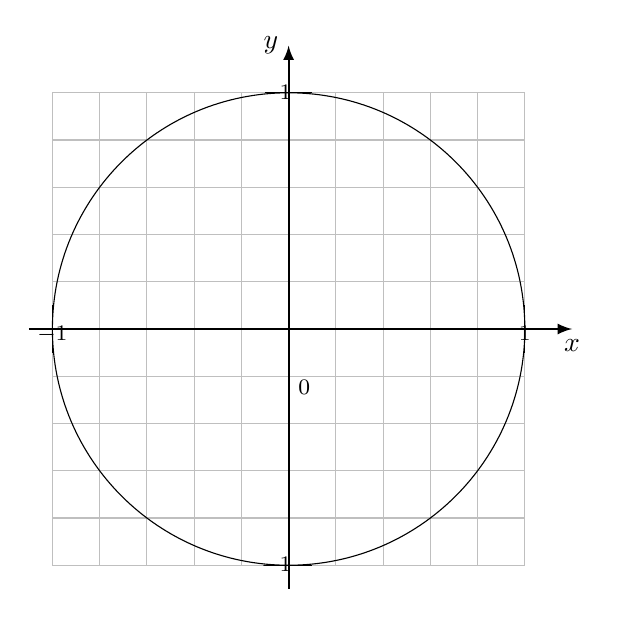
\begin{tikzpicture}[cross/.style={draw, cross out, minimum size=2*(#1-1pt), inner sep=0pt, outer sep=0pt}, x=10mm, y=10mm, 
        >=latex,   %Voreinstellung für Pfeilspitzen
        font= \footnotesize, scale=3]
        %Raster zeichnen
        \draw [color=gray!50]  [step=2mm] (-1,-1) grid (1,1);
        % Achsen zeichnen
        \draw[->,thick] (-1.1,0) -- (1.2,0) node[right, below] {\normalsize $x$};
        \draw[->,thick] (0,-1.1) -- (0,1.2) node[above, left] {\normalsize $y$};
        % Achsen beschriften
        \foreach \x in {-1,1} \draw (\x,-.1) -- (\x,.1) node[below=4pt] {$\x$};
        \foreach \y in {-1,1} \draw (-.1,\y) -- (.1,\y) node[left=4pt] {$\y$};
        % Besserer Ursprung
        \draw[color=black] (0pt,-7pt) node[right] {$0$};
        %Funktionen zeichnen:
        \clip(-1.1,-1.1) rectangle (1.1,1.1); %Bildbereich
        \draw circle [radius=1];
    \end{tikzpicture}
\end{figure}


%---------------------------------------------------------
\newpage
\question[4] % NW1 S188 A8
Welche der untenstehenden Winkel haben den gleichen Cosinuswert?
\[\frac{\pi}{2},\quad-270^\circ, \quad-120^\circ, \quad-90^\circ, \quad\frac{5\pi}{4}, \quad120^\circ, \quad135^\circ,\quad\frac{2\pi}{3}\]
Begründe mit Hilfe des Einheitskreises und ohne Verwendung des Taschenrechners.
\begin{figure}[ht]
    \begin{tikzpicture}[cross/.style={draw, cross out, minimum size=2*(#1-1pt), inner sep=0pt, outer sep=0pt}, x=10mm, y=10mm, 
        >=latex,   %Voreinstellung für Pfeilspitzen
        font= \footnotesize, scale=3]
        %Raster zeichnen
        % \draw [color=gray!50]  [step=7.5mm] (-1.3,-5.3) grid (14.8,5.8);
        % Achsen zeichnen
        \draw[->,thick] (-1.1,0) -- (1.2,0) node[right, below] {\normalsize $x$};
        \draw[->,thick] (0,-1.1) -- (0,1.2) node[above, left] {\normalsize $y$};
        % Achsen beschriften
        \foreach \x in {-1,1} \draw (\x,-.1) -- (\x,.1) node[below=4pt] {$\x$};
        \foreach \y in {-1,1} \draw (-.1,\y) -- (.1,\y) node[left=4pt] {$\y$};
        % Besserer Ursprung
        \draw[color=black] (0pt,-7pt) node[right] {$0$};
        %Funktionen zeichnen:
        \clip(-1.1,-1.1) rectangle (1.1,1.1); %Bildbereich
        \draw circle [radius=1];
    \end{tikzpicture}
\end{figure}


%---------------------------------------------------------
\newpage
\question[3] % GZP 14 A9
Es gilt: \[\sin{(\alpha)}=\frac{4}{5}.\]
Berechne \begin{parts}
    \part $\cos{(\alpha)}$ \part $\tan{(\alpha)}$
\end{parts}
ohne den Winkel $\alpha$ explizit zu berechnen.
\vspace{7pt}
\antwort{18}


%---------------------------------------------------------
\newpage
\question[4] % GZP 14 A15
\begin{minipage}{0.575\linewidth}
    Ein Aussichtsturm steht $30$m vom diesseitigen Kanalufer entfernt. Von der Aussichtsplattform $S$ aus erscheint das diesseitige Kanalufer untereinem Winkel von $\alpha=24.5^\circ$ und das jenseitige unter dem Winkel $\beta=64^\circ.$\vspace{5pt}
    \begin{parts}
        \part Wie hoch ist der Aussichtsturm?
        \part Wie breit ist der Kanal?
    \end{parts}
\end{minipage}
\hfill
\begin{minipage}{0.4\linewidth}
    \centering
\includegraphics[scale=0.5]{Trigonometrie/data-trigo/Aussichtsturm.png}
\end{minipage}
\vspace{7pt}
\antwort{18}


%---------------------------------------------------------
\newpage
\question[3] % GZP 14 A17
Im rechtwinkligen Dreieck $ABC$ mit Hypothenuse $c$ sind die Seite $a=6$ und die Seitenhalbierende $s_a=13$ gegeben. Berechne die Höhe $h_c$.
\vspace{5pt}
\antwort{22}
\end{questions}
\end{document}